\chapter{Problemanalyse}\label{ch:analyse}
\section{Administation og IT i virksomheder}

Det bliver vigtigere for virksomheder at benytte IT redskaber til administrativt arbejde og til at få virksomheden til at fungere. Uden IT falder virksomheder bagud, da de ikke kan klare opgaverne lige så effektivt som deres konkurrenter. Væsentligheden af benyttelse af IT kan beskrives som \textit{alfa og omega} \citep{case_green_team}. Desuden kan IT systemer bruges til mange forskellige administrative opgaver og færre processer gør at det bliver nemmere for ledelsen at udføre dem \citep{Ibiz_streamline}. Ved brug af IT systemer, i stedet for manuelt eller på papir, kan tal og information's integritet desuden sikres. Således ender personalet ikke med at få for lidt i løn, kunder får de rigtige varer, ting ligger de rigtige steder på lageret osv. \citep{Ibiz_streamline}. Ved at benytte et system der tjekker om dataerne er korrekte, kan virksomheden både spare tid og penge \citep{case_green_team}. Dog skal det bemærkes at cloud computing ikke er den perfekte løsning. Dropbox, en cloud storage service, er et eksempel. På deres hjemmeside står det at de stræber efter \textit{100\% uptime} men at \textit{det er urealistisk at garentere det} \citep{drpbx_downtime}. Ved brug af cloud computing er det vigtigt at være opmærksom på den downtime servicen el.lign. har. Nogle services kan f.eks. have noget downtime i løbet af ugen, hvis de skal vedligeholde noget.

Uanset hvilken sektor og branche en virksomhed befinder sig i, sker der en stigning i brug af IT som set på figur \ref{fig:virksomcc}. Figuren viser stigningen af \textit{Virksomheder der anvender cloud computing} fra år 2012 til 2014. Selvom cloud computing ikke er den eneste form for IT, står den for over en tredjedel af IT løsningerne der er, og er derved ikke ubetydelig. Derfor kan vi uddrage vigtige information af IT-brug fra Dansk Statistik data om cloud computing \citep{itvirk}.

\begin{figure}
    \centering
    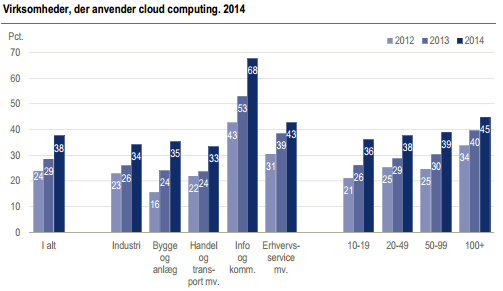
\includegraphics[width=1\textwidth]{figures/virksomhederderanvendercc.png}
    \caption{Statistik over virksomheder, som benytter cloud computing \citep{itvirk}.} 
    \label{fig:virksomcc}
\end{figure}

\begin{figure}
    \centering
    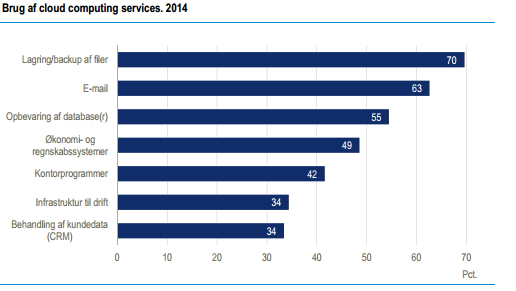
\includegraphics[width=1\textwidth]{figures/brugafccservices.png}
    \caption{Statistik over distribution af Cloud Computing brug \citep{itvirk}}
    \label{fig:distcc}
\end{figure}

På figur \ref{fig:distcc} vises det, at over halvdelen af virksomhederne, bruger cloud computing til ting som filhåndtering og database brug, samt e-mail som også påtager næsten to tredjedele af alt cloud computing brug i virksomheder. Yderligere vises det at over en tredjedel benytter det til infrastruktur, kundedata, økonomi mm. Cloud computing har den fordel, at det er allestedsnærværende. Uanset hvor en medarbejder befinder sig, enten på arbejde eller derhjemme, er der mulighed for at arbejde. I toget, derhjemme eller til møde, det er altid muligt at tilgå sine dokumenter, e-mails, applikationer osv.
Når man implementere nye it systemer er det vigtigt at man har styr på at de fungere optimalt Der er tilfælder hvor nye IT systemer ikke har fungeret optimalt. Dette kan man se på systemer som fx ”amanda” eller ”EFI” som kostede staten over 1 milliard kroner, uden at blive sat i brug\todo{[kilde]}.
I takt med at mindre virksomheder udvider samt den konkurrence imellem virksomheder, er der stigende krav til kvantiviteten og tempoet hos administrationen i virksomhederne. Denne ekstra belastning kan resultere i dårlige arbejdsforhold, hvilket vil sænke produktiviteten yderligere. Et it-værktøj til at afhjælpe i adminstrationsdelen ville kunne lette en sådan belastning og dermed højne arbejdsmiljøet\citep{It_armil}. 

%\section{Hvorfor mindre virksomheder ikke udvider}
%Der eksisterer en del mindre virksomheder indenfor byggebranchen, mange af dem vælger ikke at blive større, når håndværkermesteren indtjener det han gerne vil. Udover det virker administrationen for mange af de små virksomheder som uoverskuelig. De vælger ikke at udvide pga. manglende overskuelighed med hensyn til administration. Flere af dem frygter at miste overblikket over deres administration, hvis de udvider deres virksomhed og ansætter flere. I stedet vælger de at beholde deres størrelse, som en virksomhed på én til fire personer %\citep{SmaaFirmaerOrker}.
%I 2012 blev der indført en ny lov, som skræmte små virksomheder yderligere fra at udvide. Denne lov ville give virksomheder, som ikke havde administrationen i orden, bøder.\todo{Skal der bare stå bøder eller skal det omformuleres?} Denne lov rammer især de små virksomheder %\citep{Nyeadmboder}.
%Et eksempel på en type virksomhed, som ikke udvider, er håndværkervirksomheder. Tre ud af fire af disse virksomheder har kun én til fire ansatte. Dette skyldes som nævnt før, at de frygter administrationen af flere ansatte end dem de allerede har. De fleste af disse virksomheder er ofte ejet af en dygtig håndværker, hvor administration ikke er en del af personens %kompetencer \citep{SmaaFirmaerOrker}. \todo{Afsnittet skal generelt kigges på}


\section{Arbejdsmiljø}
\noindent Mangel på IT administration kan have stor negativ påvirkning på en arbejdsplads, og skabe et ineffektivt arbejdsmiljø. Videncenter for arbejdsmiljø har lavet en definition på begrebet arbejdsmiljø som lyder således: \textit{Arbejdsmiljø er et samspil af de relationer, påvirkninger og vilkår, som mennesket arbejder under. Det er også den tekniske og sociale udvikling af arbejdspladsen, som kan bidrage til det enkelte menneskes sikkerhed på kort sigt samt til menneskets fysiske og psykiske sundhed på længere sigt.} \citep{Arbejdsmiljoe}.

Et arbejdsmiljø kan have mange forskellige påvirkninger på arbejderen. Eksempler på disse kan være: 
\begin{itemize}
    \item {\textbf{Psykisk påvirkning} \citep{Arbejdsmiljoe_psykisk}}
    \begin{itemize}
    \item {\textbf{Stress}: At arbejde  kan være stressende, og dette kan have indvirkning på både arbejderen og arbejdsmiljøet. Stress kan f.eks. give hukommelsesbesvær, koncentrationsbesvær og nedsat humør. Disse faktorer kan både påvirke arbejderens arbejdsproces og arbejderens arbejdsomgivelser \citep{Arbejdsmiljoe_stress}.}
    \end{itemize}
    \item {\textbf{Fysisk påvirkning} \citep{Arbejdsmiljoe_fysisk}}
    \begin{itemize}
    \item {\textbf{Slid}: Et arbejde kan være fysiskt hårdt på mange måder. Dårlige muse anordninger til computerbrug kan f.eks. resultere i skader i håndled \citep{Arbejdsmiljoe_fysisk}.}
    \item {\textbf{Støj}: En larmende arbejdsplads kan også have stor indvirkning på arbejderens hørelse, i form af fysiske høreskader, men er også en faktor til psykisk stress \citep{Arbejdsmiljoe_stoej}.}
    \item {\textbf{Klima}: Aspekter som for høj eller for lav temperatur(højere end 25 grader, lavere end 20 grader), og et indelukket eller forurenet klima, kan have fysisk påvirkning på medarbejderen i form af f.eks. tørre øjne, træthed og hovedpine \citep{Arbejdsmiljoe_indeklima}.}\\
    \end{itemize}
\end{itemize}

Med henblik på IT administration, kan den negative påvirkning forekomme, når der er en mangel på effektiv IT administration, som f.eks. over-krævende- og uflexible arbejdsplaner, hvilket kan resultere i stress hos den enkelte medarbejder\citep{Cambridge2011}.

\subsection{Vagtplanens indflydelse på arbejdsmiljø}
For at forebygge konsekvenserne af et dårligt arbejdsmiljø, er en struktureret eller fleksibel vagtplan en mulighed. En fleksibel vagtplan, hvor medarbejderen er med til at vælge sine vagter, vil udover at skabe en større medarbejdertilfredshed også ansvarliggøre medarbejderen. En fleksibel vagtplan vil sikre et bedre arbejdsmiljø, ved at skabe større fleksibilitet mellem arbejde og privatliv. Det øgede ansvar giver også medarbejderen en forståelse for arbejdsplanlægningen og dermed skabe et større engagement, i at få arbejdsplanen til at gå op. Samtidig vil vagtplanlæggeren få mere tid til andet arbejde som f.eks. kvalitetssikring.
Undersøgelser viser også, at gode og fleksible arbejdstider er fastholdelses potentiale for medarbejderne, hvilket vil sige at kontinuiteten opretholdes. 
Det næste afsnit tager udgangspunkt i artiklen: \textit{Ny fleksibel arbejdstid gav mere arbejdsglæde}
\citep{Thomse2014}.

På et plejehjem i år 2010 blev der implementeret et IT-system, hvor medarbejderne selv skulle vælge sine vagter. Ifølge artiklen blev IT-systemet indført fordi \textit{Baggrunden var, at man gerne vil forebygge overbelastning af de stadig færre, der vælger at arbejde i sektoren og dermed også både fastholde dem i jobbet og rekruttere nye.} IT-systemet har givet medarbejderne mere frihed, fordi at muligheden for selv at vælge vagter, gør det lettere at tilpasse sig. Systemet virker ved at medarbejderne starter i en ønske fase, hvor de vælger de tider og dage de helst vil arbejde. Herefter bliver ønskerne puslet sammen i fællesskab, sådan at der altid er et tilstrækkeligt antal medarbejdere på arbejdet. Plejehjemmet udmelder at i denne sammenhæng, kan det være fornuftigt at have en blanding af medarbejdere der har, og ikke har børn. Denne flexible IT løsning reducerer også de mistænkelige sygedage (dage hvor man betvivler folks sygedom), fordi at medarbejderne selv fik mulighed for at vælge, hvilke dage de ville have fri. Den generelle stemning på arbejdspladsen er også blevet væsentligt bedre, da medarbejderne selv har valgt deres vagter, hvilket gør det svært at være utilfreds med arbejdstiderne. IT-systemet har derimod ikke kun været godt. I starten forholdte nogle af medarbejderne sig konservativt til løsningen og var tilfredse med vagtsystemet som de havde før. Efterhånden begyndte næsten alle dog at kunne se fordelene ved det nye IT-system. 

\section{Interessentanalyse}

Med henblik på et givet problem, så vil der være interessenter, der er interesserede i en løsning der kan løse det givne problem. Herved bliver interessentanalysen brugt til at finde de interessenter, der kunne være interesserede i at løse problemer angående ineffektiv administration og IT i små virksomheder, med henblik på planlægning.
Interessentanalyse bruges til at undersøge et problems interessenter og hvilke personer der har interesse for løsningen af dette problem, samt hvilken indflydelse de har på vigtige detaljer i løsningen. Derfor er denne analysemodel nyttig til at identificere de vigtigste interessenter, sådan at der tages forbehold for interessernes ønsker og eventuelle parter, som kunne ønske at have en negativ indflydelse på produktet. Efter at interessenterne er identificeret gennem brainstorming, bliver de placeret i en Påvirkning og Indflydelse Matrix, som lægger interessenterne i fire kategorier. En generel model af matrixen kan ses på figur \ref{fig:PåvirkInflydMat}. Interessenter placeret i det øverste venstre hjørne hører under gruppen \textit{Gidslerne}. Det er interessenter som har lille indflydelse på løsningen af problemet, men hvis samarbejde alligevel er nødvendig hvis processen skal blive en succes. Det er ofte personer der benytter et produkt, som kan blive forbedret ved hjælp af en løsning, der befinder sig i denne kvadrant. Derfor er medarbejderne placeret her, da de benytter sig af en vagtplanløsning, men ikke selv har en indflydelse på hvordan løsningen bliver udformet. De benytter sig blot af løsningen. Nederst til venstre er de \textit{Eksterne interesseressenter}. Dette er interessenter som ikke bidrager med en aktiv medvirken, eller har indflydelse på løsningen af problemet og er derfor ofte interessenter udenfor firmaet. Derfor er it-leverandører, staten og kunderne placeret i denne kvadrant. De har ikke en direkte indflydelse på udfaldet af løsningen og har heller ikke nogen indflydelse på hvordan problemet bliver løst. Øverst til højre er \textit{Ressourcepersonerne}. Denne gruppe består af personer som har stor indflydelse og medvirken i problemløsningen. Det er ofte personer som har erfaringer med kravene til det nye system, samt hvordan dette skal implementeres. Derfor placeres arbejdsplanlæggerne  her, da det er dem som har erfaring med hvordan firmaet normalt lægger deres arbejdsplan og hvilke funktioner et program skal have, for at forbedre den hidtidige procedure. Den nederste højre kvadrant er de grå eminencer, som repræsenterer de personer som har stor indflydelse på løsningen af problemet, men som ikke deltager aktivt i alle problemløsningens detaljer. Chefer er placeret i dette felt, da de kan godkende eller afslå vigtige beslutninger omkring problemløsningen, men samtidigt ikke medvirker aktivt i alle beslutninger. De kan dog vælge at gribe ind, hvis dette bliver nødvendigt.

\begin{figure}
    \centering
    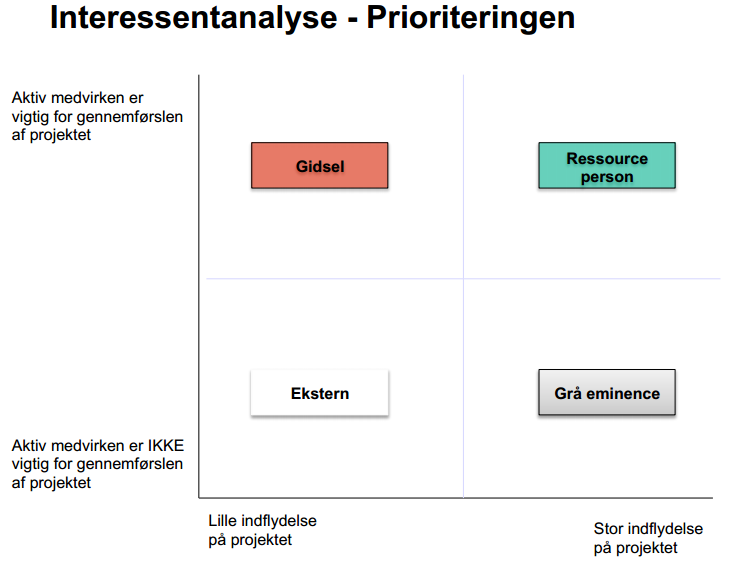
\includegraphics[width=1\textwidth]{figures/Udklip.PNG}
    \caption{Påvirkning og Indflydelse Matrix \citep{Holgaard2014}.} 
    \label{fig:PåvirkInflydMat}
\end{figure}

\subsection{Interessenter}
\textbf{Medarbejdere:}
Medarbejdere er interesseret i en løsning på problemet grundet, at de kommer til at benytte løsningen i forbindelse med deres arbejde. Deres samarbejde er vigtig for gennemførelsen af løsningen, da implementeringen afhænger af medarbejdernes samarbejdsvillighed. Selvom deres deltagelse er vigtig, har de ikke nogen indflydelse på løsningens udformning, da det oftest vil være en chef, som står for arbejdsplanlægningen og dermed bruger de blot den gennemarbejdede arbejdsplan. Medarbejdernes holdninger til projektet kan variere alt efter hvilken erfaring de har med det nuværende system. Det kan f.eks. være problematisk at skulle sættes ind i et nyt system, hvis de lige har lært at bruge det nuværende. Dog kan det også være at løsningen tilvejebringer en bedre måde for dem at håndtere deres arbejdsplan , hvorved de får mere overblik over deres arbejdstider.\\

\textbf{Chef:}
Chefen har stor interesse i løsningen af problemet, da det primært er dem som holder overblik over medarbejderne og sørger for at de kommer til tiden. Derfor kunne de være interesserede i et struktureret skema, til at holde overblik over medarbejderne. Bedre struktur kan også gøre det muligt for chefen at holde styr på hvor meget den individuelle medarbejder arbejder, sådan at reglerne om arbejdstid overholdes\todo{Tænker vi refererer til afsnittet, når vi har lavet det?}.\\

\textbf{Arbejdsplanlægger:}
Arbejdsplanlæggeren er vigtig for udviklingsprocessen, da det er denne person, som har stor erfaring med det nuværende system og kender behovene for arbejdsplanlægningen. Herved kan denne person forklare de krav og behov som arbejdsplanlægningen kræver. På dette grundlag, har arbejdsplanlæggeren en stor indflydelse på problemløsningen. Yderligere er det vigtigt at personen aktivt medvirker i løsningen af problemet for at dette bliver en succes. \\

\textbf{IT-leverandør:}
IT-leverandøren er det firma som sælger eller eksporterer et IT-produkt til virksomheden. De sælger produkter som computere, telefoner eller lignende, som skal hjælpe virksomheden med dens administration.
IT-leverandøren , har ikke stor indflydelse på løsningen og har heller ikke en vigtig medvirken i gennemførelsen af løsningen. De sørger dog for udstyr som kan bruges af virksomheden efter produktet er blevet udviklet.\\

\textbf{Kunderne:}
Kunderne for firmaet er også en interessent, da de modtager den service som firmaet tilbyder og er derfor direkte påvirkede af firmaets effektivitet. Kunderne er brugere af firmaet, men de har ikke nogen indflydelse eller medvirken på problemløsningen. De bliver indirekte påvirket af løsningen, hvilket er grunden til at de ikke har nogen indflydelse på udformningen af løsningen.\\

\textbf{Staten:}
Staten er en interessant. De er interesserede i at mindske stress på arbejdsmarkedet. Dette prøver de at gøre ved hjælp af deres kampagne \textit{Fra stress til trivsel\citep{Arbejdsmiljoe_Arbejdspladser}.} Staten er derfor interesseret i midler der kan mindske stress på arbejdsmarkedet. På dette grundlag kan det konstateres at staten kun er interesseret i det færdige produkt. De har hverken indflydelse eller medvirken i løsningen af problemet.

\section{Det kvalitative interview}
Det kvalitative forskningsinterview forsøger at forstå verden fra informantens synspunkt, herunder meninger og holdninger. Viden i forskningsinterviewet skabes i interaktionen mellem interviewer og informant. Interview er valgt frem for et spørgeskema, da den viden man får ved et interview, ikke nødvendigvis ville opstå i en spørgeskemaundersøgelse. Interview giver informanten mulighed for at fordybe sig i og udforske egne oplevelser og meninger. Den viden der opnås ved et interview, er socialt konstrueret, da det ikke bare er en dataindsamling, men at der skabes data gennem den førnævnte interaktion \citep{kvale2009}.\\

Ved hjælp af interessentanalysen, er det blevet klargjort, hvilke personer der kunne være interesserede i en løsning. Ved interviewene stræbes der efter at opnå en viden omkring hvilke problemer der er ved nuværende løsninger, samt krav til fremtidige løsninger. Interviewet blev herefter brugt til at skabe indsigt indenfor emnet. Spørgsmålene blev lavet på baggrund af nogle emner der skulle belyses. Udfra disse emner, blev nogle korte og åbne spørgsmål lavet, for at sikre, at den viden der opstod blev reflekteret over. Dette ville ikke være muligt med f.eks. ledende spørgsmål, hvor man risikerer at påvirke informanten i en bestemt retning. Ved hjælp af svarene fra interviewene blev det gjort klart, hvilke problemer der var med de nuværende systemer, samt positive sider heraf. Udfra disse data kunne en foreløbig kravspecifikation dannes.
\\
\subsection{Sammendrag af interviews}
Der blev foretaget seks interviews hos Home, KIWI, Netto, Friluftsland, Subway og Rema 1000. Denne variation af butikker er valgt, da et produkt gerne skulle laves med henblik på alle typer af SMV. Dermed er der forskellige behov fra forskellige typer virksomheder. Udfra disse interviews, er der fundet nogle styrker og svagheder frem ved nuværende systemer;\\

\textbf{Fordele:}
\begin{itemize}
\setlength\itemsep{0.3em}
\item Synkronisering til egen kalender
\item Tilgå systemet fra nettet
\item Automatisk udregning af løn til medarbejdere
\item Tjekke om medarbejdere møder til tiden
\item “Byttebørs”, hvor medarbejdere kan bytte vagter
\item Tidskrævende uden et vagtplanlægningssystem
\item Dokumentation for hvem eller hvis der blev byttet vagter\\
\end{itemize}

\textbf{Ulemper:}
\begin{itemize}
\item Manglende brugervenlighed
\item Problematisk at erstatte en tidligere medarbejder med ny
\item Butikschefen kan ikke tilgå programmet via andre platforme
\end{itemize}

Disse punkter kan anvendes til at udforme en kravsspecifiaktion. Målet med interviewene var hermed, at skaffe information omkring nuværende løsninger og dermed finde frem til, hvad en mulig løsning i dette projekt skulle indeholde. Udfra interviewene er der også blevet belyst eksisterende løsninger, som der herefter er blevet undersøgt.
Alle interviews er blevet foretaget personligt af os, og en direkte transskribering af disse, kan findes i appendix ().

\section{Teknologivurdering}

En teknologivurdering klarlægger de negative og positive konsekvenser der kan være ved en teknologi samfundsmæssigt. Der bliver udviklet teknologi til at løse problemer, men dette kan også medføre ny problemer. Det er derfor vigtig at have en grundig forståelse af problemstilling med den allerede eksisterende teknologi, så man kan udvikle en løsning med mindst konsekvenser\citep{ProTek}.
I projektet er der blevet undersøgt systemer, der hjælper med vagtplanlægning; Tamigo og Planday, samt andre mulige løsninger, som ikke er specifikt målrettet til dette problem. Denne undersøgelse bestod af at identificere hvad nuværende løsninger er i stand til, samt at bestemme fordele og ulemper ved disse løsninger. Udfra disse informationer kan der bestemmes foreløbige krav til en mulig løsning til projektet.

\subsection{Tamigo}
Tamigo er et online vagtplanlægningsværktøj som har flere forskellige funktioner. Disse funktioner tillader bl.a. administratoren at planlægge effektivt efter de gældende timeregler. Deltidsarbejderne har desuden mulighed for at bytte deres vagter og anmode om fridage online sådan at arbejdsgiveren kan bevare overblikket.\\

\textbf{Fordele: }
\begin{itemize}
\item {\textbf{Timeantal:} Tæller medarbejdernes timer og advarer arbejdsgiveren hvis antallet overskrides eller undermineres.}
\item {\textbf{Vagtbytning:} Vagtbytnings funktionen indbygget dokumentation af ændringer der bliver lavet.}
\item {\textbf{App:} Apps til smartphones som tillader medarbejderne at se planen online.}
\item {\textbf{Telefonliste:} Programmet og appen indeholder en telefonliste over medarbejderne som gør kontakt mellem arbejder og arbejdsgiver nemmere.}\\
\end{itemize}

\textbf{Ulemper: }
\begin{itemize}
\item {\textbf{Internetforbindelse:} Kan ikke ses uden internetforbindelse.}
\item {\textbf{Uoverskuelig:} Kan virke uoverskuelig hvis ikke man er blevet sat ind i systemet \citep{Tamigo, Trustpilot}.}
\end{itemize}


\todo{interview en fra en tamigo butik sådan at vi har noget info at skrive på}

\subsection{Planday}
Planday er en online vagtplan udbyder, som kan tilgås igennem platforme som f.eks. computere, tablets og mobiltelefoner. Planday har mange funktioner. Eksempler på disse er:
\begin{itemize}
\item {\textbf{Sygemelding:} Man kan melde sig syg online. Derefter kan vagtplanlæggeren se at vedkommende er syg. Vagtplanlæggeren kan herved trykke på den syges vagt og se hvilke medarbejdere der er ledige med samme kvalifikationer som den syge, og derefter vælge medarbejdere. De valgte medarbejdere vil så få en besked eller mail, om vedkommende gerne vil overtage vagten.}
\item {\textbf{Forum:} Planday tilbyder et forum. I dette forum kan chefen og alle virksomhedens medarbejdere kommunikere med hinanden, f.eks. med henblik på at bytte vagter, ferieplanlægning osv.}
\item {\textbf{Oversigt over timeantal:} Der kan ses hvor mange timer der er arbejdet, og hvor meget løn der er berettiget.}
\item {\textbf{Kundeservice:} Planday er behjælpelige når der opstår problemer hos brugeren. Når de får dårlige anmeldelser, så skriver de en hjælpende kommentar til anmeldelsen.} 
\end{itemize} 
\citep{DanskInternetHandel, Simonsen2014, Planday}\\

\noindent Ud fra brugeranmeldelser lavet omkring Planday, er der også fundet negative aspekter ved Planday. Eksempler på disse er:
\begin{itemize}
\item {\textbf{Effektivitet:} Plandays browserversion er mere effektiv end appen.} 
\item {\textbf{Utilregnelig:} Appen crasher nogle gange ved opstart.}
\item {\textbf{Information:} Den kan heller ikke altid vise de beskeder man modtaget og man kan ikke se om ens ferie er godkendt.} 
\item {\textbf{Tilgængelighed:} Kan ikke tilgås uden en online platform-} \end{itemize}
\citep{Play}\\

\subsection{Synkronisering}
Et andet eksempel på en vagtplanlægningsløsning er synkronisering til kalendere. Det fungerer ved at personen som udarbejder vagtplanen benytter programmet til at generere en fil som indeholder information omkring de ansattes mødetider. Denne fil er gemt i en standardiseret ical\todo{Daniel - forklar hvordan det virker.} format eller lignende og bliver derefter distribueret til et andet kalendersystem som f.eks. Microsoft Outlook eller Google Calander. Hver gang filen bliver ændret sendes en ny version til kalendersystem og dermed bliver medarbejdernes vagtplan regelmæssigt opdateret \citep{stage2005}. Da systemet eksporterer kalenderen til et andet system har de ansatte ikke mulighed for at ændre i den globale udgave af vagtplanen. Denne løsning har den fordel at medarbejderne ikke nødvendigvis skal sætte sig ind i et nyt program da kalenderprogrammerne er alment kendte. \todo{Skal bruge friluftsland kilde} Medarbejderne kan derved let tilgå vagtplanen selv med en ikke konstant internetforbindelse da kalenderen synkroniserer på de tidspunkter hvor der er adgang til nettet. Kalenderen kan desuden også synkroniseres til flere enheder på en gang og er derved let at tilgå. Synkronisering kan dog også foregå ved at arbejdsgiveren udgiver en vagtplan som placeres på en aftalt webadresse som medarbejderne kan tilgå. Problemet med dette er dog at medarbejderne selv skal tilgå filen fra deres enheder hver gang de skal se vagtplanen hvilket kræver at de har en netforbindelse.\\

\subsection{Manuel planlægning}
På trods af at der er mange vagtplanlægnings programmer er der stadig virksomheder, som der manuelt planlægger deres vagtplaner\todo{Kilde til Subway interview}. Der er to måder at se på dette. Den ene er at det tager meget lang tid at planlægge vagtplanen uden specialiseret software. Hvis virksomheder ikke benytter sig af software specielt til vagtplanlægning, er det ofte Microsoft Excel, der anvendes. \todo{Kilde subway interviw} Vagtplanen kan så som regel findes i printet papirform efter den er lavet, men kun der og på chefens computer. Ombytningen skal så ske uden for systemet, hvorved der manuelt skal ændres i løn og arbejdstimer, hvilket tager endnu mere tid. Ser man derimod på den anden side af manuel planlægning, så skal chefen ikke sættes ind i et nyt system. For medarbejderne gælder det samme, de skal ikke til at lære et nyt system. Virksomheden skal desuden ikke betale for nyt software (evt. med Excel som undtagelse). Der ligger altid en kopi af vagtplanen på kontoret som medarbejderne bare kan lave en personlig kopi af. Om virksomheder benytter specialiseret software eller gør det manuelt er 


%Der er stadig virksomheder da har en gammeldags tilgang til vagtplanlægning
%En statestik kunne være godt. Nogle tal (ved ikke hvilke) tag et billede af et stykke papir om nødvendigt.
%Fordele og ulemper ved papir og excel
%Sparer dog Penge, tid til at lære systemet - Se på det objektivt


%\subsection{Lectio}
%\todo {Er det relevant?}
%Lectio er et planlægningsværktøj som primært bliver brugt på gymnasier mellem lærere og elever. Servicen gør det muligt for lærere at lave et tilrettelagt skema som eleverne kan tjekke online. Udover det kan lærerne også dynamisk aflyse og flytte lektioner. Lectios anden primære funktion gør det muligt for den enkelte elev at uploade opgaver til Lectios servere hvor der bliver holdt styr på elevens totale afleveringsprocent samt fysisk fravær \citep{Macom}.

\section{Problemafgrænsning}
\begin{itemize}
\item Afgræns problemet - Bl.a. synkronisering til kalender er >MÅSKE< ikke noget vi kan lave tidsmæssigt og det er ikke så datalogisk interessent da det er simpelt < Hvis det er simpelt, vorfor har vi så ikke tid til at lave det ?

\end{itemize}


\section{Problemformulering}